\begin{framed}

Objetivos:
\begin{itemize}
    \item Describir las diferentes escalas de movimiento en un flujo turbulento.
    \item Encontrar la escala de Kolmogorov.
    \item Presentar los principales modelos para simular la turbulencia. 
\end{itemize}

Contenidos:
\begin{itemize}
    \item Escalas de movimiento.
    \item La energía cinética y disipación
    \item La cascada de energía.
    \item La escala de Kolmogorov.
    \item Los modelos de turbulencia.
\end{itemize}

Bibliografía:
\begin{itemize}
    \item White, F. M. (2006) Viscous fluid flow. McGraw-Hill. Tercera edición. Capítulo 6.7
    \item Bernard, P. S. and Wallace, J. M. (2002) Turbulent Flow. Analysis, Measurements, and Prediction. John Wiley \& Sons. Sección 2.6.
\end{itemize}
\end{framed}

\section*{Escalas de movimiento}

Hagamos el siguiente experimento mental: digamos que tenemos un vaso con agua, la cual revolvemos con una cuchara.
En la macro escala, uno esperaría que la cuchara empuje al fluido y este comience a moverse en una trayectoria circular, similar a la de la cuchara.
Esa intuición es correcta, sin embargo, si nos acercamos, nos podremos dar cuenta que el paso de la cuchara no solo genera un movimiento en la escala del movimiento de la cuchara, si no que además genera pequeños vórtices que se desprenden del flujo ``grande''.
Luego, si nos acercamos aún más, veremos que esos vórtices generan escalas de movimiento aún más pequeñas, y así sucesivamente.
Por lo tanto, a pesar que nosotros estamos introduciendo un flujo del porte de la cuchara y las vueltas que damos para revolver, finalmente estamos generando vórtices de muchas escalas.

Estos vórtices más pequeños ocurren por la inestabilidad del flujo laminar. 
De hecho, si revolviésemos suficientemente lento las perturbaciones en las otras direcciones serían aplacadas por la viscosidad, y no tendríamos vórtices más pequeños.
Esto nos dice que esta distribución de escalas de movimiento es una indicación de turbulencia, y resulta en el flujo aparentemente desordenado del que hemos estado conversando.

En esta clase vamos a estudiar esta cascada de escalas, y veremos que es lo que ocurre en cada una de ellas.

\section*{Energía cinética y disipación}

La clase pasada introdujimos el concepto de energía cinética turbulenta:
%
\begin{equation}
K = \frac{1}{2}\overline{u'_iu'_i},
\end{equation}
%
que corresponde a la energía cinética debido a las fluctuaciones en la velocidad.
Por otra parte, presentamos una ecuación de conservación de la energía cinética turbulenta, la cual es:
%
\begin{align}\label{eq:K_conservacion}
\frac{DK}{Dt} =& -\frac{\partial}{\partial x_i} \left[ \overline{u'_i\left(\frac{1}{2}u'_iu'_j+\frac{p'}{\rho}\right)}\right] - \overline{u'_iu'_j}\frac{\partial\overline{u}_j}{\partial x_i} \nonumber\\
               & + \frac{\partial}{\partial x_i}\left[\overline{\nu u_j'\left(\frac{\partial u'_i}{\partial x_j} + \frac{\partial u_j'}{\partial x_i}\right)}\right] -\nu\overline{\frac{\partial u_j'}{\partial x_i}\left(\frac{\partial u_i'}{\partial x_j}+\frac{\partial u_j'}{\partial x_i}\right)},
\end{align}
%
y describimos el significado físico de cada uno de los términos.
Detengámonos en el último de ellos, que llamamos disipación:
%
\begin{equation}\label{eq:disipacion}
\epsilon_T = \nu\overline{\frac{\partial u_j'}{\partial x_i}\left(\frac{\partial u_i'}{\partial x_j}+\frac{\partial u_j'}{\partial x_i}\right)}.
\end{equation}
%
Este término es el responsable de la disipación de la energía cinética en forma de calor, mediante fricción molecular. 
Podemos descomponer la disipación en dos términos:
%
\begin{align} \label{eq:disipacion_iso}
\epsilon_T &= \epsilon + \nu\overline{\frac{\partial u_i'}{\partial x_j}\frac{\partial u_j'}{\partial x_i}} \text{, donde,} \nonumber \\
\epsilon &= \nu\overline{\left(\frac{\partial u_j}{\partial x_i}\right)^2},
\end{align}
%
y a $\epsilon$ lo llamamos la disipación isotrópica.
De hecho, en el caso de turbulencia homogénea homogénea, el término $\overline{\frac{\partial u_j'}{\partial x_i}\frac{\partial u_j'}{\partial x_i}}= \frac{\partial}{\partial x_j}\left(\overline{u_i\frac{\partial u_j}{\partial x_i}}\right) = 0$, y $\epsilon_T=\epsilon$.

\paragraph*{La función de correlación.}
A continuación intentaremos dilucidar la escala a la cual ocurre la disipación.
Esta es una derivación bastante más larga de lo que presentamos acá, pero intentaremos de darle sentido sin entrar en demasiados detalles.

Definamos una función $R_{ij}(\mathbf{x},\mathbf{y},t) = \overline{u'_i(\mathbf{x},t)u'_j(\mathbf{y},t)}$ que llamamos la función de correlación entre dos puntos.
Esta función de correlación no es más que el promedio de la multiplicación de la velocidad evaluada en dos puntos $\mathbf{x}$ y $\mathbf{y}$, y nos entrega información de que tanto cambian las fluctuaciones de velocidad en el espacio; si un flujo es extremadamente desordenado y turbulento, es muy probable que $R_{ij}$ sea muy cercano a cero, y en general, uno esperaría que se alejara de cero a medida que $\mathbf{x}$ e $\mathbf{y}$ se acerquen.
Fíjense que $R_{ii}$ para $\mathbf{x}\to\mathbf{y}$ no es más que dos veces la energía cinética ($2K$).

Pensemos que estamos hablando de turbulencia homogénea isotrópica (sus propiedades son homogéneas en el dominio, y no dependen de la dirección).
En este caso, es intuitivo pensar que la correlación $R_{ij}$ no depende de los puntos absolutos $\mathbf{x}$ y $\mathbf{y}$, si no que de la distancia entre ellos $\mathbf{r} = \mathbf{y}-\mathbf{x}$.
De esta forma, podemos definir una función de correlación $R'_{ij}$ tal que $R'_{ij}(\mathbf{r},t) = R_{ij}(\mathbf{x},\mathbf{y},\mathbf{t})$, y sus derivadas son:
%
\begin{align}
\frac{\partial R_{ij}}{\partial x_k} &= -\frac{\partial R'_{ij}}{\partial r_k} \nonumber \\
\frac{\partial R_{ij}}{\partial y_k} &= \frac{\partial R'_{ij}}{\partial r_k} \nonumber\\
\frac{\partial^2 R_{ij}}{\partial x_k^2} &= \frac{\partial^2 R_{ij}}{\partial y_k^2} = -\frac{\partial^2 R_{ij}}{\partial x_k\partial y_k} = \frac{\partial^2 R'_{ij}}{\partial r_k^2} 
\end{align}
%
Si derivamos $R_{ij}$ con respecto a $\mathbf{x}$ e $\mathbf{y}$, llegamos a
%
\begin{equation}
\frac{\partial^2R_{ij}}{\partial x_k\partial y_k} = \frac{\partial}{\partial x_k}\frac{\partial}{\partial y_k} R_{ij} =\frac{\partial}{\partial x_k}\frac{\partial}{\partial y_k} \overline{u'_i(\mathbf{x},t)u'_j(\mathbf{y},t)} = \overline{\frac{\partial u'_i}{\partial x_k}\frac{\partial u'_j}{\partial y_k}} = -\frac{\partial^2 R'_{ij}}{\partial r_k^2},
\end{equation}
%
lo que es igual a $\epsilon/\nu$.
De esta forma encontramos una relación entre la energía cinética turbulenta y la disipación isotrópica, ya que $R'_{ij}(\mathbf{r}=0) = 2K$, y $\frac{\partial^2 R'_{ij}}{\partial r_k^2}(\mathbf{r}=0) = \frac{\epsilon}{\nu}$.

\paragraph*{Turbulencia en el espacio de Fourier.}
Podemos descomponer una función como una expansión infinita de transformadas de Fourier.
Por ejemplo, la descomposición de Fourier de $R_{ij}'(\mathbf{r},t)$ es
%
\begin{equation}\label{eq:expansion_fourier}
R_{ij}'(\mathbf{r},t) = \int_0^\infty \hat{R}_{ij}(\mathbf{k},t)e^{ik\mathbf{r}}d\mathbf{k},
\end{equation}
%
y la pregunta se reduce a encontrar la función $\hat{R}_{ij}(\mathbf{k},t)$, tal que esa integral represente a la función original fielmente.
Afortunadamente, tenemos la transformada de Fourier para calcular ese término:
%
\begin{equation}\label{eq:transformada_fourier}
\hat{R}_{ij}'(\mathbf{k},t) = \int_0^\infty R_{ij}(\mathbf{r},t)e^{-ik\mathbf{r}}d\mathbf{r}.
\end{equation}
%
\mbox{?`}Para qué sirve todo esto? Quizás es más fácil visualizarlo en forma discreta: pensemos que en vez de una integral tenemos una suma (la integral puede ser vista de esta manera).
Fíjense que el término $e^{ik\mathbf{r}}=\cos(kr)+i\sin(kr)$ es una suma de un seno y un coseno, donde $k$ es el número de onda (o frecuencia espacial).
Por lo tanto, la expansión de Fourier en la Ec. \eqref{eq:expansion_fourier} puede ser visto como una suma de senos y cosenos de diferente frecuencia, y $\hat{R}_{ij}(\mathbf{k},t)$ es la constante que acompaña a cada seno y coseno.
De esta forma, podemos pensar que para representar una función que varía muy lento, proablemente encontremos que $\hat{R}_{ij}(\mathbf{k},t)$ son altos para $\mathbf{k}$ pequeños.
Por otra parte, para una función que varía muy rápido en el espacio, los factores $\hat{R}_{ij}(\mathbf{k},t)$ que dominen van a ser de $\mathbf{k}$ altos.

Así podemos ver la utilidad de la transformada de Fourier en la Ec. \eqref{eq:transformada_fourier}, ya que nos indicará la naturaleza de la función: es de ``alta'' o ``baja'' variabilidad.
Volvamos a hablar de mecánica de fluidos.
Dijimos anteriormente que al revolver un vaso de agua generamos movimientos en muchas escalas, la más grande es la escala del giro de la cuchara, y que se generarían vórtices cada vez más pequeños.
En término relativos, la escala grande varía ``lento'' en el espacio, y mientras más chica la escala, más ``rápida'' es la variación.
Si hacemos una descomposición de Fourier del flujo, las escalas grandes excitarán los $\mathbf{k}$ más pequeños, y los vórtices chicos los $\mathbf{k}$ más grandes.
Por lo tanto, si $l_e$ es la longitud característica de un vórtice, $\l_e\sim 1/k$.
Un ejemplo: un flujo laminar solo tiene una escala de movimiento, por lo que excitaría solo un $\mathbf{k}$ (o un pequeños conjunto de $\mathbf{k}$s que están muy cerca uno de otro).

Para encontrar la expansión de Fourier de la energía cinética, solamente debemos hacer $i=j$ en la Ec. \eqref{eq:transformada_fourier} y evaluar $\mathbf{r}=0$ (pues $\mathbf{x}\to\mathbf{y}$), y llegamos a
%
\begin{equation}\label{eq:K_fourier}
K(t) = \int_0^\infty \hat{R}'_{ij}(\mathbf{k},t)d\mathbf{k}
\end{equation}

Encontrar la transformada de Fourier de la derivada de una función es muy fácil. 
Derivemos la Ec. \eqref{eq:expansion_fourier}:
%
\begin{align}
\frac{\partial R_{ij}'}{\partial r_i}(\mathbf{r},t) &= \int_0^\infty \hat{R}_{ij}(\mathbf{k},t)\frac{\partial}{\partial r_i}e^{ik\mathbf{r}}d\mathbf{k} = \int_0^\infty ik\hat{R}_{ij}(\mathbf{k},t)e^{ik\mathbf{r}}d\mathbf{k}\nonumber\\
\frac{\partial^2 R_{ij}'}{\partial r_i^2}(\mathbf{r},t) &= \int_0^\infty \hat{R}_{ij}(\mathbf{k},t)\frac{\partial^2}{\partial r^2_i}e^{ik\mathbf{r}}d\mathbf{k} = \int_0^\infty -k^2\hat{R}_{ij}(\mathbf{k},t)e^{ik\mathbf{r}}d\mathbf{k},
\end{align}
%
por cada derivada, simplemente multiplicamos por $ik$ para encontrar la transformada de Fourier!
Ya encontramos la relación entre la energía cinética turbulenta y la disipación isotrópica, donde $R'_{ij}(\mathbf{r}=0) = 2K$, y $\frac{\partial^2 R'_{ij}}{\partial r_k^2}(\mathbf{r}=0) = \frac{\epsilon}{\nu}$.
Por lo tanto, la transformada de Fourier asociada a la disipación es igual a la transformada de Fourier de la energía cinética, multiplicada por $k^2$.
Entonces podemos escribir una expansión de Fourier para la disipación:
%
\begin{equation}\label{eq:disipacion_fourier}
\epsilon(t) = -\nu k^2 \int_0^\infty \hat{R}'_{ij}(\mathbf{k},t)d\mathbf{k}
\end{equation}

Pensemos bien en lo que nos dice la Ec. \eqref{eq:disipacion_fourier} en comparación con la Ec. \eqref{eq:K_fourier}.
Imaginen que tenemos un flujo turbulento del cual conocemos su campo de velocidades, calculamos su energía cinética y la transformada de Fourier $\hat{R}'_{ij}$.
Esta transformada de Fourier nos indicará cuales son los $\mathbf{k}$ más excitados, por ejemplo, en la Figura \ref{fig:energia_fourier}, el peak de $\hat{R}'_{ij}$ ocurre en $k_d$.
Pero al multiplicarlo por $k^2$ el peak se corre hacia la derecha, y ahora se encuentra en $k_e$
\mbox{?`}Qué significa esto? Que la disipación a alto $k$, o sea, en los vórtices más pequeños.
%
\begin{figure}[h!]
\centering
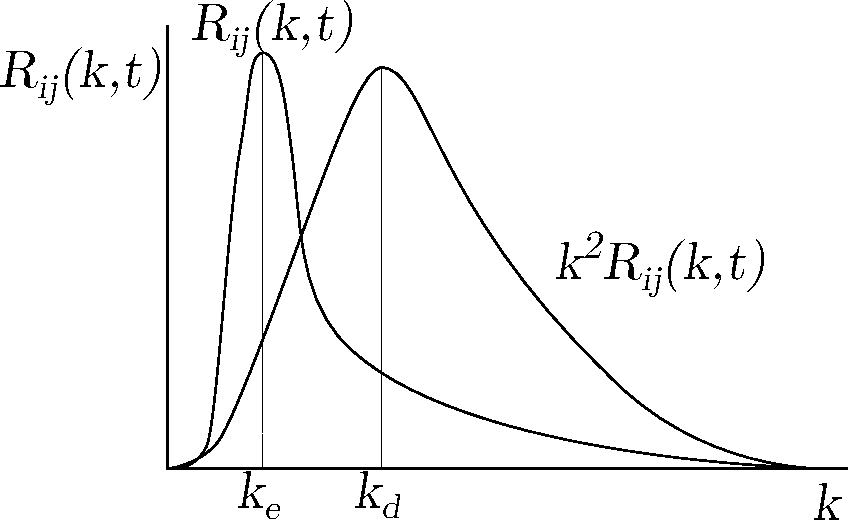
\includegraphics[width=0.6\textwidth]{clase03/energia_fourier.pdf}
\caption{Gráfico de energía con respecto a escalas de movimiento}
\label{fig:energia_fourier}
\end{figure}

Aquí ocurre algo interesante: mientras la energía cinética entra al sistema por las grandes escalas (la cuchara que revuelve), la disipación de energía cinética ocurre en las pequeñas escalas.
Esto nos dice que tiene que haber un mecanismo de transferencia de energía cinética desde los vórtices grandes a los pequeños, en lo que se llama la \emph{cascada de energía}.

\section*{La cascada de energía y escalas de movimiento}

\subsection*{La escala de Kolmogorov}
La forma en que la energía cinética entra al flujo es a través de la cuchara, por lo que se hace intuitivo que la energía cinética se inyecta en la escalas grandes de movimiento.
La pregunta ahora es, \mbox{?`}En que escala ocurre la disipación? En otras palabras, \mbox{?`}cuanto es $k_d$ en la Figura \ref{fig:energia_fourier}?
Una estimación de esta escala se la debemos a Andrey Komogorov.
En su analisis, Komogorov supone que el flujo de escalas pequeñas, alejado de cualquier borde, tiene un carácter universal.
Esto es, a pesar de que el flujo en las escalas grandes es claramente dependiente de la naturaleza del flujo (por ejemplo, flujo en tubería, chorro, etc.), cuando uno se fija solamente en las escalas pequeñas, la fuente de la energía cinética es irrelevante.
A esas escalas, sea un flujo en tubaría, chorro, o una cuchara revolviendo un vaso, el flujo es equivalente.
Y como ya vimos antes, es en estas escalas donde ocurrirá la disipación, lo que transfiere la energía cinética a calor gracias a la viscosidad.

A partir de esta suposición, Kolmogorov usó principios del análisis dimensional para encontrar $k_d$.
En las escalas pequeñas, los únicos parámetros relevantes son la disipación (que contiene la velocidad), la viscosidad (que transfiere la energía cinética a calor), y el tamaño de los vórtices ($\eta$).
Podemos decir entonces que el tamaño de los vórtices más pequeños debe ser función de $\epsilon$ y  $\nu$ solamente, y por análisis dimensional, la única forma de obtener unidades de longitud es con
%
\begin{equation}\label{eq:l_kol}
\eta = \left(\frac{\nu^3}{\epsilon}\right)^{1/4}.
\end{equation}
%
donde $\eta\sim\frac{1}{k_d}$, y $\eta$ se conoce como la escala de Kolmogorov.

Un flujo laminar tiene solamente una escala, y en esta escala la difusión es la que domina.
De esta forma, podemos hacer el paralelo con la escala de Kolmogorov para decir que un flujo turbulento puede ser visto como una colección de pequeños flujos laminares, y por tanto, la escala de Kolmogorov es la escala más pequeña de movimiento.

Usando este mismo principio, el tiempo característico del flujo en esta escala (o escala temporal de Kolmogorov) es:
%
\begin{equation}\label{eq:t_kol}
t_d = \left(\frac{\nu}{\epsilon}\right)^{1/2}
\end{equation}

A pesar que la derivación de estas ecuaciones parece ser poco rigurosa, si es una muy buena estimación.
De hecho, hay resultados experimentales que demuestran que la mayor parte de la disipación ocurre para escalas $k<0.5/\eta$.

\subsection*{La escala inercial}
Ya hemos conversado de las grandes escalas ($k_e$), donde la energía cinética es creada, y las pequeñas escalas ($k_d$), donde la energía cinética es disipada.
\mbox{?`}Qué ocurre entonces entre $k_e$ y $k_d$ en la Figura \ref{fig:energia_fourier}?
Este sector intermedio se conoce como la escala inercial. 
En la escala inercial no hay producción ni disipación importante de energía cinética, ya que, como aparece en la Figura \ref{fig:energia_fourier} los peaks de producción y disipación no se encuentran en esta región.
La escala inercial solamente transfiere la energía de las grandes escalas (donde se produce) a las pequeñas escalas (donde se disipa).
Usemos nuevamente el análisis dimensional para estudiar como se comporta la energía en esta región, sabiendo que en este caso, la viscosidad no es importante.
Primero, sabemos que la disipación tiene unidades de $[\epsilon] = L^2/S^3$ y que el número de onda tiene unidades de $[k] = 1/L$.
Además, la transformada de Fourier en la Ec. \eqref{eq:K_fourier} ($\hat{R}'_{ij}$) debe tener unidades de energía dividido por número de onda ($K/k$), que da $L^3/T^2$.
De esta forma, la única manera en que se pueden relacionar estos valores para que tengan sentido dimensional es
%
\begin{equation}\label{eq:energia_inercial}
\hat{R}'_{ij}(k) = C_K k^{-5/3}\epsilon^{2/3}
\end{equation}
%
donde $C_K$ se conoce como la constante de Kolmogorov.
Nuevamente, a pesar que esta derivación parece ser poco rigurosa, experimentalmente se ha visto que la energía cae con $k$ como lo predice la Ec. \eqref{eq:energia_inercial}, y normalmente $C_K=1.4$ funciona bastante bien.
Con esta nueva información, podemos completar la Figura \ref{fig:energia_fourier} con el rango inercial, como lo muestra la Figura \ref{fig:energia_inercial}.
Esta transferencia de energía desde las grandes a las pequeñas escalas se conoce como cascada de energía. 
%
\begin{figure}[h!]
\centering
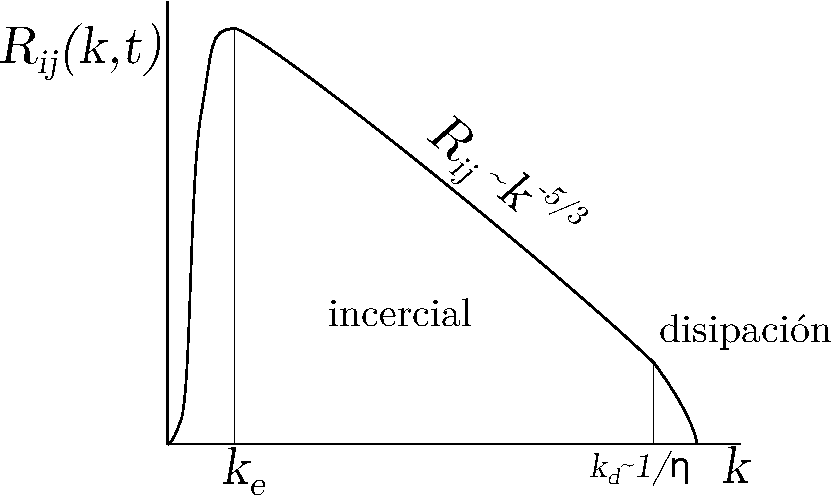
\includegraphics[width=0.8\textwidth]{clase03/energia_inercial.pdf}
\caption{La cascada de energía en escala logarítmica.}
\label{fig:energia_inercial}
\end{figure}

La interpretación más física de la cascada de energía esta representada por la Figura \ref{fig:escala_vortice}, donde la energía cinética es producida por los vórtices grandes (por ejemplo, generados por una cuchara que revuelve un vaso de agua), luego es transferida a las pequeñas escalas a través del rango inercial, y finalmente se disipa en los pequeños vórtices por viscosidad.
%
\begin{figure}[h!]
\centering
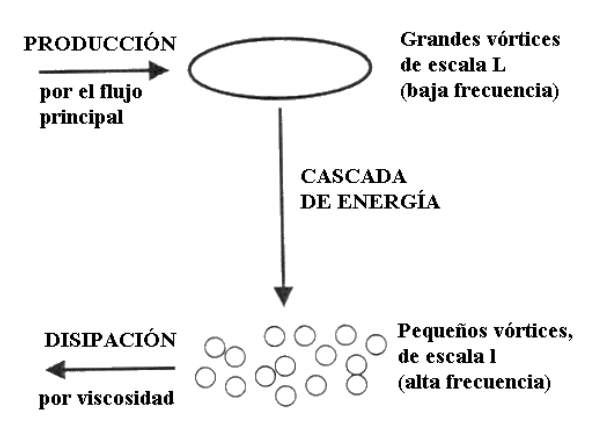
\includegraphics[width=0.6\textwidth]{clase03/escala_vortice.png}
\caption{Interpretación de la escala de energía.}
\label{fig:escala_vortice}
\end{figure}

\subsection*{La escala de Kolmogorov y el número de Reynolds}

Pensemos en la energía cinética turbulenta y la disipación en términos de la conservación.
Si hay energía cinética turbulenta disipándose, es porque esta fue generada en las grandes escalas.
Esta idea nos permite decir que debe una relación entre la disipación y las variables en las grandes escalas.
Usemos, nuevamente, análisis dimensional para encontrar tal relación.
En las grandes escalas, las variables importantes son la longitud característica de los grandes vórtices ($l$), y la velocidad ($v$).
Por análisis dimensional, la única forma de obtener disipación a partir de estos valores de la ``macro'' escala es
%
\begin{equation}\label{eq:disipacion_macro}
\epsilon\sim\frac{u}{l}.
\end{equation}
%
Juntando la Ec. \eqref{eq:disipacion_macro} con la Ec. \eqref{eq:l_kol}, llegamos a:
%
\begin{align}\label{eq:disipacion_Re}
\eta &= \left(\frac{\nu^3}{\epsilon}\right)^{1/4} \sim \left(\frac{\nu^3 l}{u^3}\right) = l\left(\frac{\nu^3}{u^3l^3}\right)^{1/4} \nonumber\\
\Rightarrow & \frac{\eta}{l} \sim \left(\frac{\nu}{ul}\right)^{3/4} = Re^{-3/4}.
\end{align}

Esto nos entrega una nueva interpretación del número de Reynolds.
Normalmente se presenta como el ratio entre fuerzas inerciales y fuerzas viscosas, sin embargo, también puede ser visto como el ratio entre las pequeñas y grandes escalas.
Este resultado tiene profundo efecto en la simulación numérica de fluidos (CFD), ya que, para simular correctamente un flujo, la malla debe ser lo suficientemente fina como para resolver de buena forma hasta las escalas más pequeñas del flujo.
La Ec. \eqref{eq:disipacion_Re} nos permite estimar el número de nodos que necesitaremos. 
Por ejemplo, si la escala del problema es 1m, el número de nodos que necesitaremos es $1/\eta$, y considerando que una simulación completa implica 3 dimensiones, el número de nodos será $N=Re^{9/4}$.
Un problema muy simple: una persona ($l\sim 2$m) trotando ($v\sim 5$m/s) en aire ($\nu\sim10^{-5}$) da un $Re\sim10^6$, o sea $N\sim10^{13}$ nodos.
Solamente para guardar la posición del nodo en la malla necesitamos 3 valores ($x, y, z$), a 4 bytes cada valor son $16\cdot10^{13}$ bytes, \mbox{!`}$160$ TBytes!
Esto hace que el desarrollo de modelos de turbulencia tenga mucho sentido.

\section*{Modelación de la turbulencia}

Como vimos recién, se hace prácticamente imposible modelar todas las escalas de un flujo turbulento para la gran mayoría de las aplicaciones interesantes de ingeniería.
Por esta razón, en vez de resolver la ecuación de Navier-Stokes completa, utilizamos la ecuación promediada de Reynolds que estudiamos la clase pasada. 
A modo de recordatorio, esta ecuación es
%
\begin{equation}\label{eq:RANS7}
\frac{\partial \overline{u}_i}{\partial t} + \overline{u}_j\frac{\partial \overline{u}_i}{\partial x_j} + \frac{\partial \overline{u'_iu'_j}}{\partial x_j} = -\frac{1}{\rho}\frac{\partial \overline{p}}{\partial x_i} + \nu \frac{\partial}{\partial x_j}\frac{\partial \overline{u}_i}{\partial x_j},
\end{equation}

Esta ecuación tiene la particularidad de ser muy parecida a la ecuación de Navier-Stokes con todos sus términos promediados, más la derivada del tensor de esfuerzos de Reynolds ($\overline{u_i'u_j'}$).
Es de hecho el tensor de esfuerzos de Reynolds la fuente de todos los problemas en la simulación de la turbulencia, y es este término el que los modelos de turbulencia intentan modelar.

Existen muchos modelos de turbulencia que se pueden separar en dos familias: simulaciones RANS, que utilizan la ecuación \eqref{eq:RANS7}, y las simulaciones con grandes vórtices (Large Eddy Simulations, LES).
En ingeniería, RANS es más utilizado que LES porque es un método más maduro, pero se considera a LES un modelo más exacto.
A continuación repasaremos algunos modelos RANS, pues es lo que más se encuentra en aplicaciones reales.

\subsection*{Modelos RANS}
Los modelos para calcular $l_m$ se clasifican en:
%
\begin{itemize}
\item Modelos de ninguna ecuación
\item Modelos de una ecuación
\item Modelos de dos ecuaciones
\end{itemize}


\subsection*{Modelos de ninguna ecuación.}
\paragraph*{La viscosidad turbulenta.}
Al poner el tensor de esfuerzos de Reynolds en la derecha de la ecuación en la Ec. \eqref{eq:RANS7}, se hace natural pensar en los efectos turbulentos como un paralelo a la viscosidad.
Para que sea más claro, conviene reescribir el tensor de esfuerzos de Reynolds de la forma
%
\begin{equation}
\rho\overline{u'_iu'_j}=\mu_t\frac{\partial \overline{u}_i}{\partial x_j}, 
\end{equation}
%
La pregunta es \mbox{?`}Cuánto es el valor de la viscosidad $\mu_t$, que reproduzca los efectos viscosos correctamente?
Lo más simple es considerar $\mu_t$ como una constante.
A pesar de que $\mu_t$ tiene dimensiones de viscosidad, este no es una propiedad del fluido, y varía dependiendo de la condición del flujo y la geometría.

\paragraph*{Longitud de mezcla de Prandtl.} Otro modelo simple es el de longitud de mezcla de Prandtl, que escribe $\mu_t$ como
%
\begin{equation}
\mu_t = \rho l_m^2\left|\frac{\partial \overline{u}_1}{\partial x_2}\right|
\end{equation}
%
donde $x_1$ corre en la dirección del flujo y $x_2$ perpendicular a él.
El término $l_m$ se conoce como longitud de mezcla, y es un valor que depende del caso que estamos analizando y el modelo a utilizar.
Usando el modelo de longitud de mezcla de Prandtl, el tensor de esfuerzos de Reynolds queda
%
\begin{equation}
\overline{u_1'u'_2} = l_m^2\left|\frac{\partial \overline{u}_1}{\partial x_2}\right|\frac{\partial \overline{u}_1}{\partial x_2}
\end{equation}

El término $l_m$ se conoce como longitud de mezcla, y es un valor que depende del caso que estamos analizando. 
Si estamos viendo turbulencia isotrópica, l m seria una constante, sin embargo, si el problema es turbulencia cerca de una pared, un buen modelo es considerar que la longitud de mezcla varía linealmente $l_m = Ky$. 
Otros casos son un chorro circular, donde $l_m$ = 0,75$\delta$, donde $\delta$ es el diámetro del chorro.

\subsection*{Modelo de una ecuación: Prandtl-Kolmogorov}
Este modelo acopla la ecuación de energía cinética turbulenta (Ec. \eqref{eq:K_conservacion}) a las ecuaciones de continuidad y cantidad de movimiento (Ec. \eqref{eq:RANS7}).
Para cerrar el modelo de Prandtl-Kolmogorov necesitamos hacer algo al respecto de $\mu_t$ y los términos de generación y disipación de energía cinética:
%
\begin{align}
\nu_t &= \frac{\mu_t}{\rho} = C_1\frac{K^{1/2}}{L} \nonumber\\ 
\epsilon &= C_2\frac{K^{3/2}}{L} \nonumber\\
\overline{-v\left(\frac{1}{2}u_i'u_i'+\frac{p'}{\rho}\right)} &= C_3\frac{\partial K}{\partial y}
\end{align}
%
donde las constantes $C_1$, $C_2$ y $C_3$ son obtenidas de experimentos.
Cabe destacar que en el modelo de Prandtl-Kolmogorov resuelve tres ecuaciones en vez de dos, lo que lo hace computacionalmente más intenso.


\subsection*{Modelos de dos ecuaciones}
En general, los modelos de dos ecuaciones son los más aceptados en términos de su exactitud, y son ampliamente encontrados en programas de modelación computacional de fluidos.
Algunos de estos modelos son
%
\begin{itemize}
\item $K-\epsilon$ con métodos de renormalización (Yakhot y Smith (1992))
\item $K-\omega$ de Prandtl
\item $K-L$ de Rotta
\item $K-\omega^2$ de Wilcox
\end{itemize}

Todos estos modelos son relativamente parecidos.
Los modelos de dos ecuaciones no solo agregan una ecuación como el modelo de Prandtl-Kolmogorov, si no que agregan una segunda ecuación, y es donde difiere cada modelo.
Por ejemplo $k-\epsilon$ agrega una ecuación para la disipación o $K-L$ para la longitud de la escala turbulenta.
Revisemos el más conocido, el $K-\epsilon$.

\paragraph*{Modelo $K-\epsilon$}
El modelo $K-\epsilon$ agrega a la Ec. \eqref{eq:K_conservacion} con las aproximaciones del modelo de Prndtl-Kolmogorov, la siguiente ecuación para la disipación
%
\begin{equation}
\frac{D\epsilon}{Dt} = \frac{\partial}{\partial x_j} \left(\frac{\nu_t}{\sigma_\epsilon}\frac{\partial\epsilon}{\partial x_j}\right) + C_1\nu_t\frac{\epsilon}{K}\frac{\partial\overline{u}_i}{\partial x_j} \left(\frac{\partial\overline{u}_I}{\partial x_j}+\frac{\partial\overline{u}_j}{\partial x_i}\right) - C_2\frac{\epsilon^2}{K}
\end{equation}
%
con
%
\begin{equation}
\nu_t = \frac{C_\mu K^2}{\epsilon}
\end{equation}
%
y las constantes
%
\begin{align}
C_\mu = 0.09 \quad C_1=1.44 \quad C_2 = 1.92 \quad \sigma_K = 1 \quad \sigma_\epsilon=1.3. 
\end{align}
%
Lamentablemente estas constantes no son universales y dependen del tipo de flujo.
